El objetivo de desarrollo de la presente librería se basa en el siguiente principio, “ cuando un elemento sea actualizado, sea un botón, cuadro de estado, entrada de texto, etc. el componente regresará un objeto el cual tendrá el nombre del elemento y el nuevo valor para que este sea actualizado en el state de react ”.  Con esto deseamos generar el siguiente flujo.
\newline
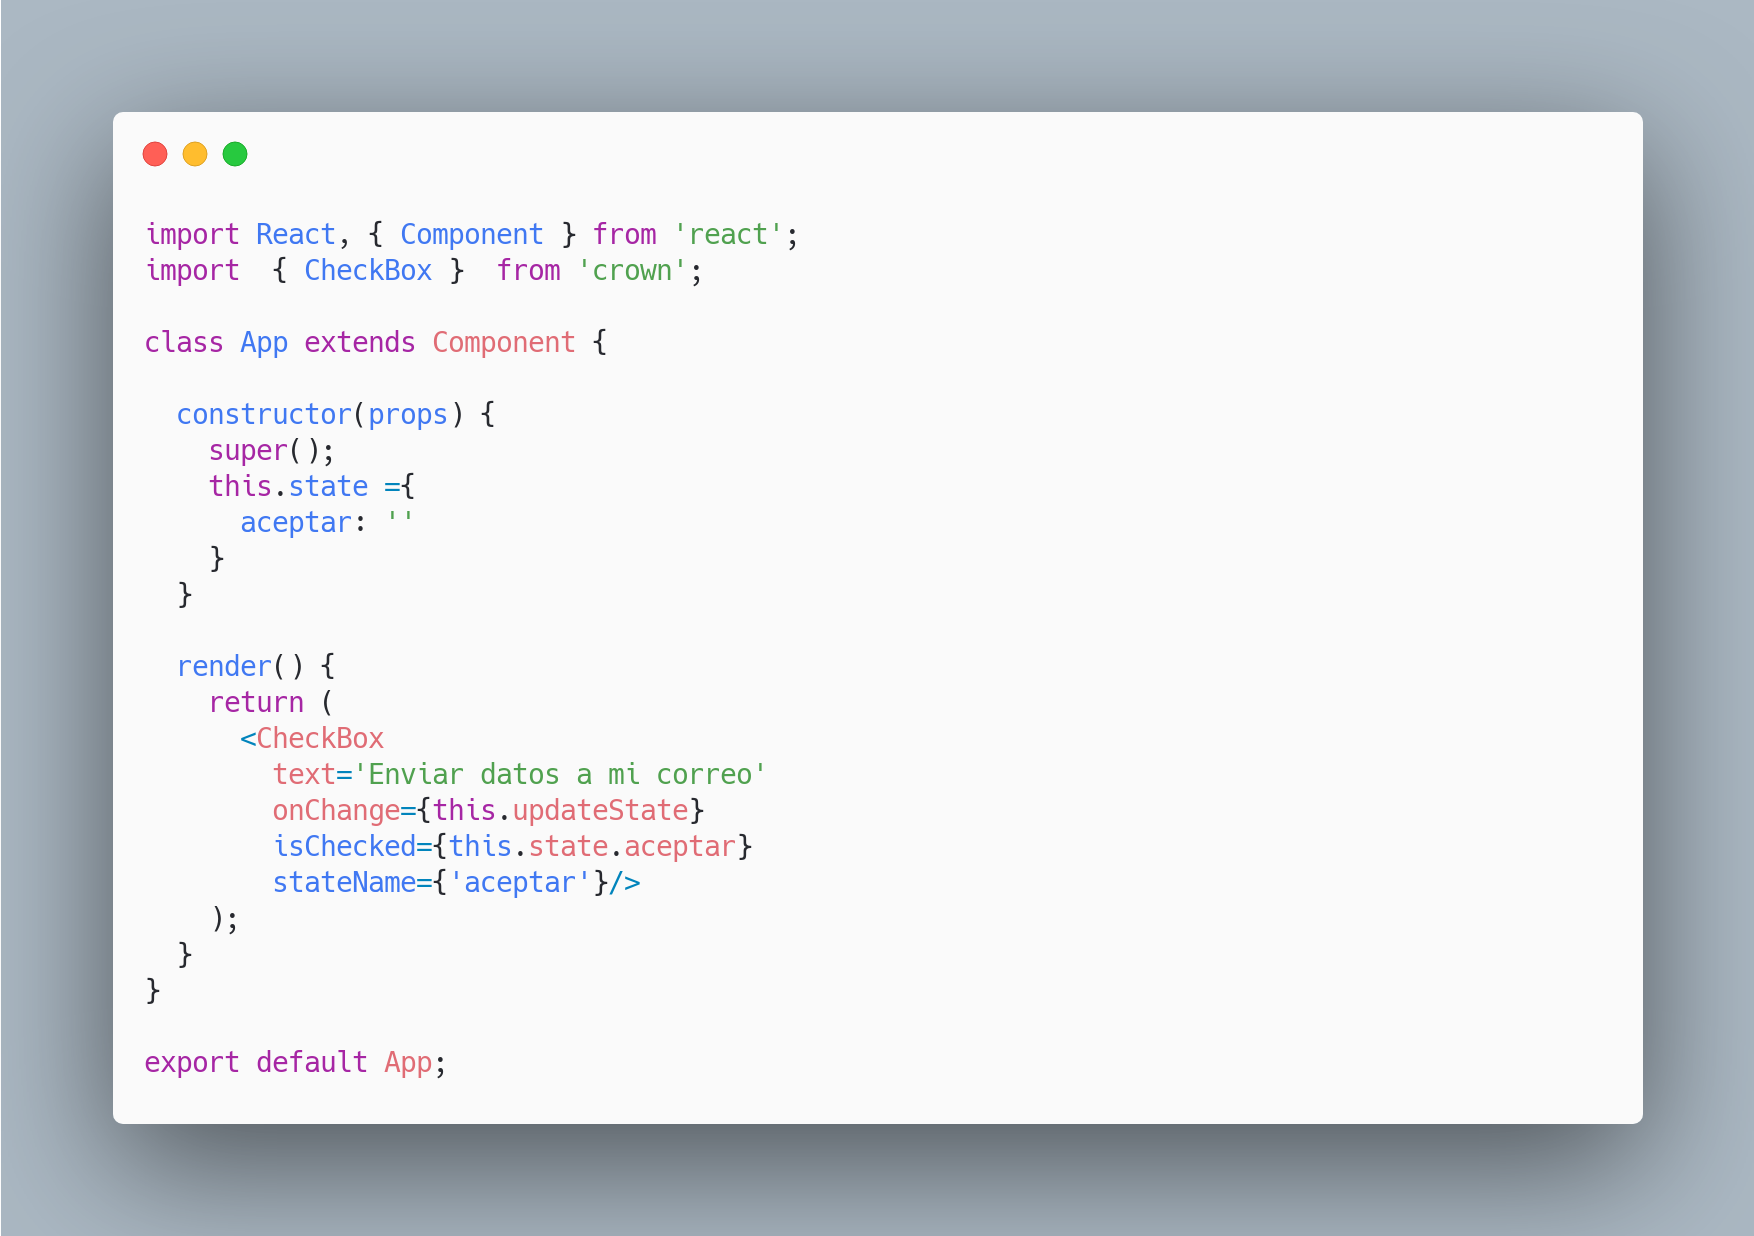
\includegraphics[width=1\textwidth]{./Imagenes/carbon-8.png}
\newline
Importamos el elemento CheckBox desde “crown” dentro de el método render en return  ponemos el componente CheckBox y le damos los  siguientes  props.

\begin{itemize}
	\item \textbf{onChange:} Función que actualiza el estado, que definiremos adelante.
	\item \textbf{isChecked::} Ponemos el valor de “aceptar” que está en el estado.
	\item \textbf{stateName:}  Es el nombre ( y no el valor como en isChecked ) con el que identificamos el elemento en el estado. 
\end{itemize}

\newline
Dentro del componente CheckBox se devuelve un objeto como el que se muestra enseguida.

\newline
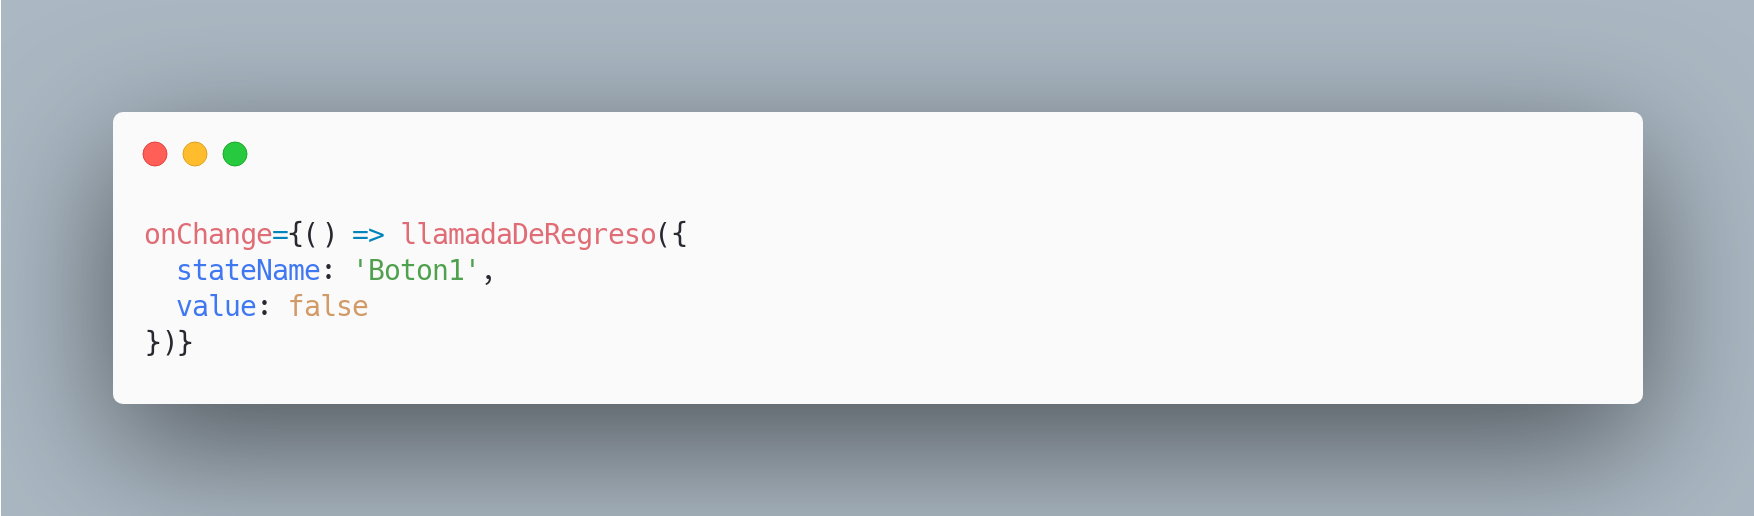
\includegraphics[width=1\textwidth]{./Imagenes/carbon-6.png}
\newline


\begin{itemize}
	\item \textbf{onChange:}  Este es el evento que se ejecuta cuando una acción es disparada, por ejemplo cuando haces click en un CheckBox.
	\item \textbf{llamadaDeRegreso:} Es la función que recibe el componente, y cuando se hace click en un CheckBox este, por defecto llama la acción que está dentro del evento onChange. En este caso llama a llamadaDeRegreso.
	\item \textbf{stateName:}  Es el nombre ( y no el valor como en isChecked ) con el que identificamos el elemento en el estado. 
	\item \textbf{value:}  Este dato almacena el valor actualizado del elemento, esto define si el CheckBox está seleccionado o no.
\end{itemize}
\newline
Esto facilitará a tener una única función capaz de actualizar todos los elemento que agregamos ya que contamos con el nombre,  que es con el que se identifica en el estado y también el nuevo valor.
\newline
\newline
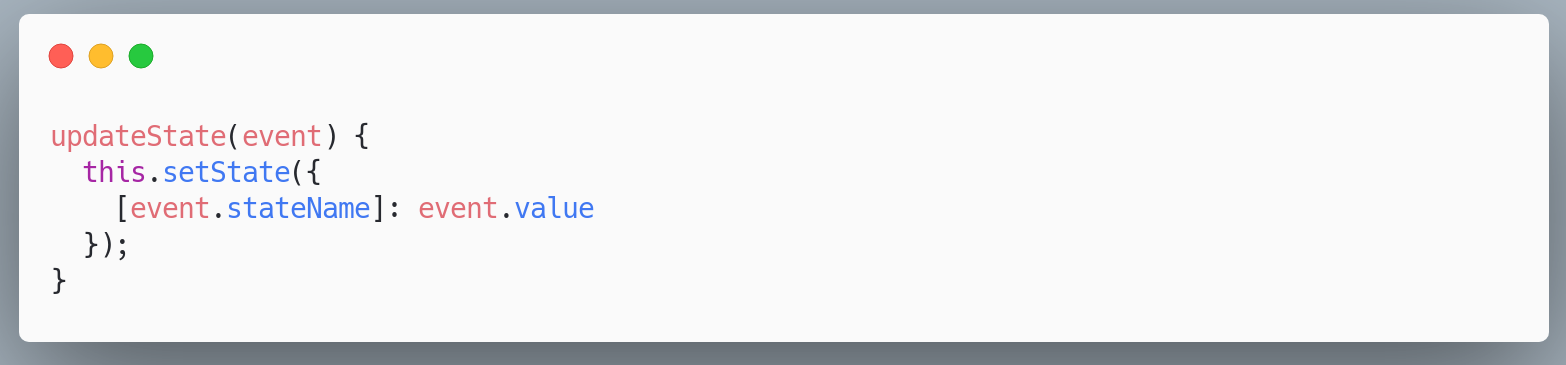
\includegraphics[width=1\textwidth]{./Imagenes/carbon-7.png}
\newline

\end{enumerate}